	The following python codes draw the graphs which are represented in Fig.\ref{fig:3.7.5_qelevena} and Fig.\ref{fig:3.7.5_qelevenb}.
	\begin{lstlisting}
	./solutions/5/codes/lines/q11a.py
	./solutions/5/codes/lines/q11b.py
	\end{lstlisting}
	\solution
	\begin{figure}[!ht]
	\centering
	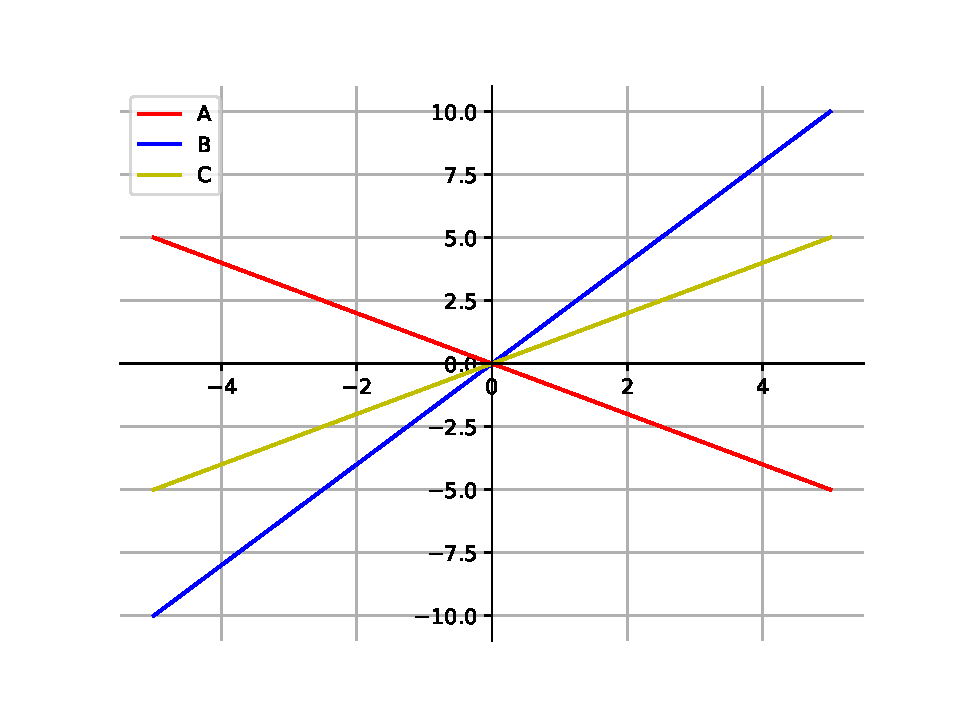
\includegraphics[width=\columnwidth]{./solutions/5/figs/lines/q11a.eps}
	\caption{}
	\label{fig:3.7.5_qelevena}	
	\end{figure}
	\begin{figure}[!ht]
	\centering
	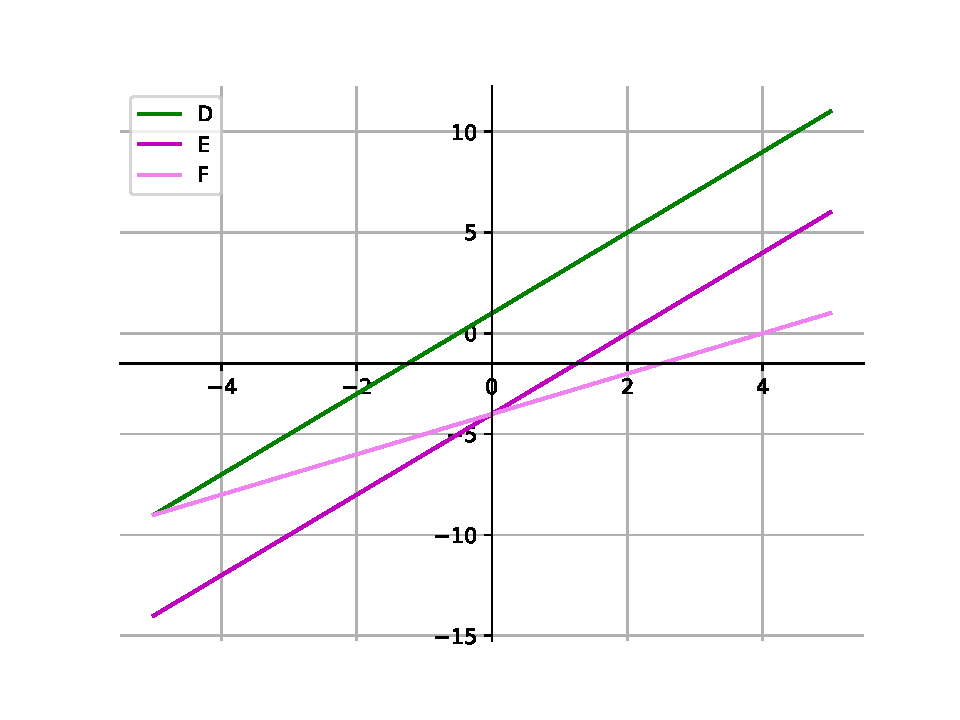
\includegraphics[width=\columnwidth]{./solutions/5/figs/lines/q11b.eps}
	\caption{}
	\label{fig:3.7.5_qelevenb}	
	\end{figure}
	
